\section{Introduction}
% What is RC. Given sufficient data good, otherwise bad.
Relation classification (RC) is an indispensable problem in information extraction and knowledge discovery. Given a sentence (e.g., \emph{Washington is the capital of the United States}) containing two target entities (e.g., \emph{Washington} and \emph{the United States}), an RC model aims to distinguish the semantic relation between the entities mentioned by the sentence (e.g., \emph{capital of}) among all candidate relation classes.

Conventional relation classification has been extensively investigated. Recent approaches \cite{zeng-etal-2014-relation,RNNRC,vu-etal-2016-combining} train models with large amount of annotated data and achieve satisfactory results.
%Recent approaches are substantially based on neural networks and
%deep learning \cite{zeng-etal-2014-relation,RNNRC,vu-etal-2016-combining},
%where the models are trained with large amount of human-annotated data
%and achieve satisfactory results.
%\KZ{What does this mean? OK}
However, it is often costly to obtain necessary amount of labeled data by human-annotation,
without which a decrease in the performance of the RC models is inevitable.
% Distant supervised ways
In order to obtain sufficient labeled data,
distant supervised  methods \cite{NYTdataset} have been adopted to enlarge annotation quantity by utilizing existing knowledge bases to perform auto-labeling on massive raw corpus. However, long-tail problems \cite{xiong-etal-2018-one,han-etal-2018-fewrel,ye-ling-2019-multi} and noise issues occur.
%The NYT-10 dataset \cite{NYTdataset} is a typical large dataset constructed under distant supervision.
%Although these approaches substantially augment labeled data,
%significant shortcomings remain: %\KZ{Elaborate a bit what you mean bylong-tail problem. OK}
%(1) Long-tail problems \cite{xiong-etal-2018-one,han-etal-2018-fewrel,ye-ling-2019-multi} exist in knowledge bases. While some particular relation classes contain a great proportion of instances, most classes consist of only tens of instances.  (2) Noise issues occur during auto-labeling, demanding for manual screening.

\begin{table}[t]
	\centering
	\small
	\caption{\label{FewShotRCExample}
		An example of 5-way 5-shot relation classification scenario from the FewRel validation set. $Entity~1$ marks the head entity, and $entity~2$ marks the tail entity. The query instance is of Class 1: \emph{mother}. The support instances of Classes 2-5 are omitted.
	}
	\begin{tabular}{p{8cm}}
		\hline
		\textbf{Support Set} \\ \hline
		\textbf{Class 1} \emph{~mother}: \\
		\qquad \textbf{Instance\;1}~\lbrack Emmy Acht\'e\rbrack$_{entity~1}$ was the mother of the internationally famouse opera singers \lbrack Aino Ackt\'e\rbrack$_{entity~2}$ and Irma Tervani. \\
		\qquad \textbf{Instance\;2}~He was deposed in 922, and \lbrack Eadgifu\rbrack$_{entity~1}$ sent their son, \lbrack Louis\rbrack$_{entity~2}$ to safety in England. \\
		\qquad \textbf{Instance\;3}~Jinnah and his wife \lbrack Rattanbai Petit\rbrack$_{entity~1}$ had separated soon after their daughter, \lbrack Dina Wadia\rbrack$_{entity~2}$ was born. \\
		\qquad \textbf{Instance\;4}~Ariston had three other children by \lbrack Perictione\rbrack$_{entity~1}$: Glaucon, \lbrack Adeimantus\rbrack$_{entity~2}$, and Potone.\\
		\qquad \textbf{Instance\;5}~She married (and murdered) \lbrack Polyctor\rbrack$_{entity~2}$, son of Aegyptus and \lbrack Caliadne\rbrack$_{entity~1}$. Apollodorus.\\
		\textbf{Class 2} \emph{~part\_of}: ... \\
		\textbf{Class 3} \emph{~military\_rank}: ... \\
		\textbf{Class 4} \emph{~follows}: ... \\
		\textbf{Class 5} \emph{~crosses}: ... \\ \hline
		\textbf{Query Instance} \\ \hline
		Dylan and \lbrack Caitlin\rbrack$_{entity1}$ brought up their three children, \lbrack Aeronwy\rbrack$_{entity2}$, Llewellyn and Colm. \\
		\hline
	\end{tabular}
\end{table}

% Few-shot RC
%\KZ{The following three paras can be merged and shortened to make some space.
%Directly attack the problems in meta learning. Move some of the intro of
%few-shot learning and meta learning to related work.}
Few-shot relation classification is a particular RC task under minimum annotated data of 
{\em concerned relation classes}, i.e., a model is required to classify an incoming query 
instance given only few support instances (e.g., 1 or 5) during testing. 
An example is given in Table~\ref{FewShotRCExample}.
%\KZ{I found this para to be puzzling. On the one hand u said minium annotated data, on the other
%hand, u said the model is actually trained with a lot of data at training time. Seems
%contradictive. How can they be so stupid to define a problem like this?}
It is worth noting that, in previous few-shot RC tasks, although models see only few support instances during testing, they are trained with a large amount of data (e.g., tens of thousands of instances in total), labeled with relation classes different from but in the same domain of the {\em concerned
relation classes}.
This situation arises when instances of several relation classes are hard to find while 
those of others are abundant.
But in practice, it is often hard to get so many annotated training data as well. 
The difficulty %of labeling abundant training data 
lies in 2 aspects:
\begin{enumerate}
	\item Expertise required. Labeling is hard when it comes to professional fields such as bio-medical and risk management instead of general corpus. The relation classes in professional fields tend to be confusing and expertise is required.
	% In domains such as medical health and risk control, the relation classes are confusing and expertise required.
	%For example, in medical health domian, it is not easy to tell if a term such as \emph{hypertension} a disease or a symptom. 
	Thus the cost of labeling increases.
	\item Useless samples. Overwhelming majority (above 90\% in some of our experiments) 
of instances are of relation class \emph{NA} (no relation). 
This situation is particularly true in domains such as bio-medical and risk management, 
where a large proportion of instances are %\KZ{This is not the right term? white samples} 
ordinary samples
but only the samples with health issues 
or risks are of our concern. This makes labeling very unproductive. 
%We can only get a handful of useful annotated instances after going through hundreds of raw samples.
\end{enumerate}
In this paper, we highlight the situation where in-domain training data is hard to obtain as is illustrated above, and restrict the size of training data in few-shot relation classification.
%Thus the original intention of few-shot learning (i.e., annotating less data) is violated.
%In this paper, we add a constraint on the size of training data to better conform to the origin intention of labeling less data.

\begin{figure}[tbh!]
	\centering
	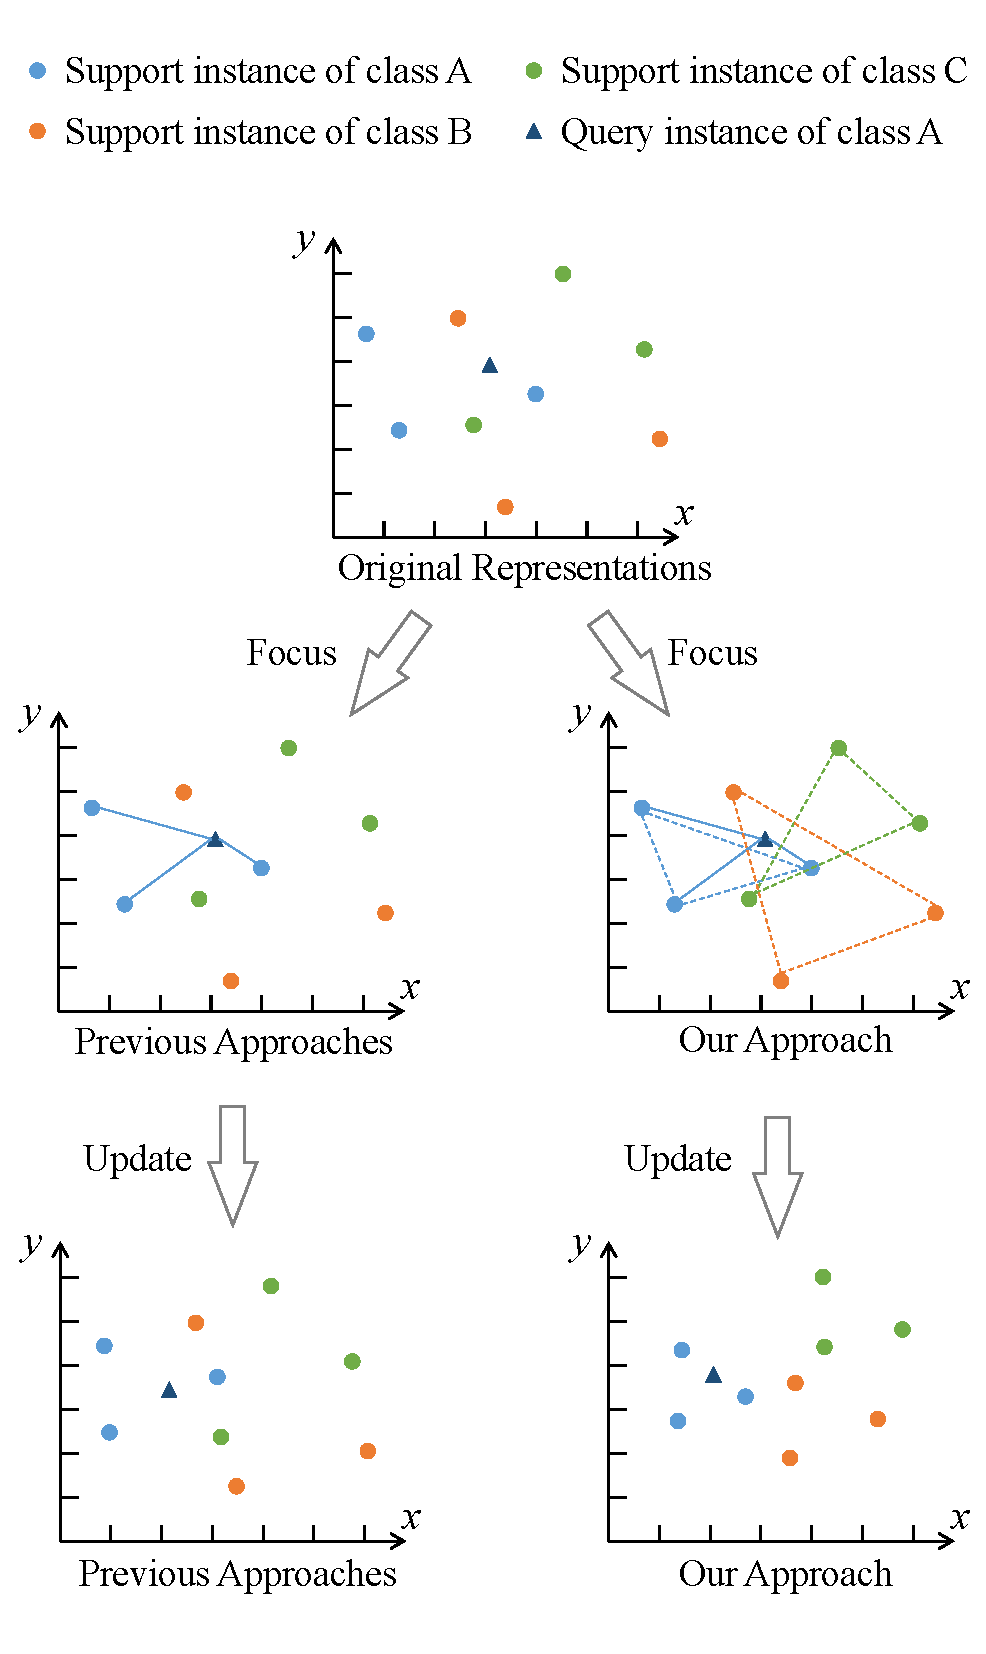
\includegraphics[width=8.5cm]{support.pdf}
	\caption{The general idea of model's updating process of one iteration. Previous approaches update the representations merely by the classification results on query instances. Our approach updates the representations by classification results on both query instances and support instances.
	%Solid lines indicate the intention of making representations of query instances and support instances closer to their target classes.
	Solid lines indicate the intention of making representations of the query instance and each support instance of the same class closer to each other.
	Dotted lines indicate the intention of making representations of support instances within each class closer.
	}
	\label{fig:support}
\end{figure}


% Meta learning
Meta-learning is a popular method for few-shot learning circumstances and is broadly studied in computer vision (CV) \cite{LakeHuman,Santoro2016,proto}.
Instead of training a neural network to learn a specific task, in meta-learning, the model is trained with a variety of similar but different tasks to gain the ability of quick adaptation to new tasks without meeting a ton of data.
One typical framework of meta-learning is to train an additional meta-learner %
%\KZ{Rephrase this: on the upper to guide the upgrading steps of the conventional learner on the lower OK}
which sets and adjusts the update rules for the conventional learner \cite{Andry2016,Finn2017,HN}. Another framework is based on metric learning and is aimed at
learning the distance distribution among the relation classes \cite{Koch2015,Vinyals2016,proto}.
% Prototypical networks \cite{proto} is a typical and widely used metric learning based meta-learning framework.
% Recent works on meta-RC
%In recent years, meta-learning has been adopted in NLP to solve few-shot learning problems, including few-shot relation classification as a focus of this paper.
In recent years, meta-learning has been shown to help in few-shot NLP tasks,
including few-shot relation classification, which is the focus of this paper.
%\cite{gu-etal-2018-meta,han-etal-2018-fewrel,huang-etal-2018-natural,obamuyide-vlachos-2019-meta,ye-ling-2019-multi}.
%In this paper, we focus on meta-learning methods for few-shot relation classification task.
Han et al. \shortcite{han-etal-2018-fewrel} constructed the FewRel dataset, a few-shot relation classification dataset and applied distinct meta-learning frameworks intended for CV tasks on the FewRel dataset. Ye and Ling \shortcite{ye-ling-2019-multi}, Gao et al. \shortcite{hatt} and Gao et al. \shortcite{gao-etal-2019-fewrel} improved the models specifically for relation classification task
and achieved better performance.
%In recent years, meta-learning has been adopted in NLP as a solution to multiple few-shot learning tasks. %\cite{gu-etal-2018-meta,han-etal-2018-fewrel,huang-etal-2018-natural,obamuyide-vlachos-2019-meta,ye-ling-2019-multi}.
%In this paper, we focus on meta-learning methods for few-shot relation classification task.
%\cite{han-etal-2018-fewrel} constructed the FewRel dataset, a few-shot relation classification dataset and first applied distinct meta-learning frameworks intended for CV tasks on the FewRel dataset. \cite{ye-ling-2019-multi,hatt,gao-etal-2019-fewrel} improved the models to cater for relation classification task and achieved better performances.
%Prototypical networks \cite{proto} with CNN encoder turned out to have the best performance. \cite{ye-ling-2019-multi} improved the framework of prototypical networks by interactively encoding the support and query instances at both local and instance level, and adding weights while calculating prototypes. \cite{gao-etal-2019-fewrel} adopted BERT \cite{devlin2018bert} in few-shot relation classification.


% What's different in our work
While meta-learning frameworks outperform conventional methods in few-shot RC, 
%there is still room for further improvement.
%One disadvantage is that previous models concern much about
%\KZ{the outputs of the query instances OK}
%computations on query instances but lose sight of information within the support instances. Besides, the requirement for significant
%amount of human annotation is not \emph{really} eliminated in previous work.
%Although just few support instances are needed during testing,
%the training set still must be sufficiently large
%(e.g., the FewRel dataset \cite{han-etal-2018-fewrel}
%contains 700 instances per relation). Performance drops significantly when
%the training data size is restricted (e.g., tens of instances per relation).
%First of all, %the requirement for significant amount of human annotation is not \emph{really} eliminated in previous work. 
they are not applicable to situations where only small amount of annotated training data is available, which does happen in practice.
In previous work, although only few support instances are needed during testing, the training set still must be sufficiently large (e.g., the FewRel dataset \cite{han-etal-2018-fewrel} contains 700 instances per class). Performance drops significantly when the training data size is restricted
(e.g., to tens of instances per relation). Strong baselines such as MLMAN \cite{ye-ling-2019-multi} and Bert-Pair \cite{gao-etal-2019-fewrel} achieves satisfactory performance (about 80\% accuracy on 5-way 1-shot tasks) with full FewRel training data, but accuracy decreases by 20\% if 10 relation classes with only 10 instances per class are given as training data (see Section \ref{results}).
Besides, previous meta-learning methods concern much about computations on query instances but lose sight of knowledge within the support instances.
Typical methods regard the features of support instances as \emph{standards} to classify query instances during training iterations.
We hold the view that improving the quality of the \emph{standards} itself
by extracting knowledge within support instances is important but
overlooked by previous work.

To %address these weaknesses, we propose
enhance models and make them better cater to small training data, we propose
%\KZ{Find another name?}
\emph{Meta-learning using Intra-support and Cross-domain Knowledge} (MICK) framework.
%Firstly, inspired by \cite{chen-2019-image}, we exploit underlying knowledge within support instances using a support classifier scheduled by a fast-slow learner (\secref{sec:cls}). Secondly, we improve the model performance by augmenting training data with open-source relation classification instances. This is quite helpful under conditions where few training data of the target domain is available (\secref{sec:data}).
First, we
%improve the model performance by introducing cross-domain knowledge. We
utilize cross-domain knowledge by enriching the training tasks with cross-domain relation classification dataset
(e.g., adding relation class \emph{mother} to a medical relation classification training set,
and forming a 3-way training task with relation classes \emph{Disease-cause-Disease}, \emph{Disease-have-Symptom}, and \emph{mother})
%augmenting training data with open-source relation classification instances to
(\secref{sec:data}).
The only requirement on the cross-domain dataset is to share the same language with the original dataset, thus it is easy to find.
Although differences exist in distributions of data from distinct domains, basic knowledge such as language principles and grammar are shared, and thus compensate for the insufficient learning of basic knowledge due to lack of training data.
%with the help of common knowledge brought by cross-domain data.
Moreover,
%cross-domain relation classification dataset enriches the training tasks.
even adding only a few cross-domain relation classes brings about a huge increase in the amount of feasible tasks. Task enrichment makes the model more reliable by forcing it to solve extensive and diverse training tasks.
%This is quite helpful under conditions where few training data of the target domain is available (\secref{sec:data}).
Second, inspired by Chen et al. \shortcite{chen-2019-image}, we exploit underlying knowledge within support instances using a support classifier scheduled by a fast-slow learner (\secref{sec:cls}).
Instead of updating the instance representations merely by classifying the query instances according to the support instances, 
we also use the support classifier to classify the support instances and update the model so that representations of support instances of the same class are closer to each other (see \figref{fig:support}). 
This makes the instance representations within the same class more compact, thus the classification of query instances becomes more accurate.
% This makes the representation of each instance more reasonable, thus improving classification accuracy.

Additionally, we propose our own dataset, TinyRel-CM dataset,
a Chinese few-shot relation classification dataset in health domain. 
Different from previous few-shot RC dataset which contains abundant training data, we purposely limit the size of training data of our dataset.
%Two primary problems exist in the previous few-shot relation
%classification dataset.  One is that 
%Previous dataset contains
%abundant training data, violating the original intention of
%``few-shot'' (i.e., utilizing small amount of data).
%Besides, in reality, if instances of some relation classes are so rare that few-shot RC is needed, it is often unrealistic to extract mass instances of other classes within the same domain and constructing a huge training set.
%But in reality, if instances of some relation classes are so rare that few-shot RC is needed, it is often unrealistic to extract mass instances for other classes within the same domain and constructing a huge training set.
%The other problem is that most of the relation classes in previous dataset are highly distinguishable because they have distinct head and tail entity types
%(e.g., \emph{mother} and \emph{part\_of}. \emph{mother}
%describes the relation between head entity \emph{PERSON1} and
%tail entity \emph{PERSON2}, while \emph{part\_of} describes that of
%head entity \emph{OBJECT1} and tail entity \emph{OBJECT2}).
%However, in practice, it is more meaningful to classify seemingly
%indistinguishable relation classes that share the same head and
%tail entity types (e.g., \emph{mother} and \emph{spouse}, where both
%head entity types are \emph{PERSON1} and both tail entity types are \emph{PERSON2}).
%Previous few-shot RC dataset contains abundant training data, which violates the original intention to use small amount of data.
%\KZ{Say why you create your own data. Must be the fewRel is not good enough?}
The TinyRel-CM dataset contains 27 relation classes with 50 instances per class, 
which sets up the challenge of few-shot relation classification under \emph{small} training data. 
This dataset
is also challenging because the relation classes in the test set are all very similar to each
other. %Moreover, the relation classes in our dataset is categorized into groups according to the head and tail entity types, and models are required to perform relation classification within each group. 
Experiments are conducted on both our proposed TinyRel-CM dataset and the FewRel dataset \cite{han-etal-2018-fewrel}. Experimental results show the strengths of our proposed framework.

 %that (1)
%%\KZ{How do you show it's a hard task? OK}
%The MSI framework with data augmentation achieves competitive results given sufficient training data. (2) Both MSI framework and the data augmentation method bring performance gains. (3) The MSI framework with data augmentation becomes more effective with less training data.

% Our contributions
In summary, our contributions include:
 (1) We propose a meta-learning framework that achieves state-of-the-art performance with the limitation of small training data and competitive results with sufficient training data (\secref{results}).
%TinyRel-CM is more challenging than FewRel because it contains extremely limited amount of training data (see \secref{dataset}).
%(2) We find that extracting knowledge within support instances benefits the meta learning process.
%(2) Knowledge within support instances improves performance. We make use of this knowledge with a support classifier (\secref{results}).
(2) We utilize a support classifier to extract intra-support knowledge and
obtain more reasonable instance representations and demonstrate the improvement (\secref{results}).
(3) We propose a task enrichment method to utilize cross-domain implicit knowledge, which is extremely useful under small training data (\secref{results}).
%(4) Our method achieves state-of-the-art performance in Chinese few-shot relation classification dataset in health domain.
(4) We propose TinyRel-CM dataset,
%a Chinese few-shot relation classification dataset in medical domain.
the {\bf second} and a challenging dataset for few-shot relation classification task with small training data (\secref{dataset} and \secref{results}).
%(4) Our methods achieve state-of-the-art performance on our proposed TinyRel-CM dataset and competitive results on the FewRel dataset (\secref{results}).

%This is the {\bf second} dataset for few-shot relation classification task.
%TinyRel-CM is more challenging than FewRel because it contains extremely
%limited amount of training data (see \secref{dataset}).
%(2) We find that extracting knowledge within support instances benefits the meta learning process. To make use of knowledge within support instances, we facilitate the meta-learning framework with a support classifier (see \secref{results}).
%(3) We propose a data augmentation method. When training data is very small, it is useful to borrow knowledge from out-of-domain data (see \secref{results}).
%(4) Our methods achieve state-of-the-art performance
%on TinyRel-CM dataset and competitive results on FewRel \cite{han-etal-2018-fewrel} dataset (\secref{results}).
%\KZ{It seems that (3) can be combined into (2) because you said TinyRel-CM
%has much fewer training data earlier. So if u do well in TinyRel-CM, it means
%you are particularly good with small training data.}
